\documentclass{article}
\usepackage{polski}
\usepackage[utf8]{inputenc}
\usepackage{graphicx}
\usepackage{amsmath}
\usepackage{amssymb}
\usepackage{mathtools}

\title{UOA LAB - Ćwiczenie 1}
\author{Jan Bronicki 249011}
\date{}

\begin{document}

\maketitle


\section{Wstęp}
Zapoznanie się z meodą wyznaczania modelu zastępczego Kupfmullera oraz Strejca. Wykreślenie wykresu charakterystyki
dynamicznej dla modelu rzeczywistego i jak najdokładniejsze odczytanie z niego parametrów modeli zastępczych.
\subsection{Wykorzystane programy w ćwiczeniu}
\begin{itemize}
    \item Matlab
    \item Python
    \item Excel
\end{itemize}

\section{Wyznaczenie modeli zastępczych}
Z otrzymanych danych wyjściowych modelu rzeczywistego będziemy tworzyć następnie charakterystyki.

\begin{figure}[h!]
    \centering
    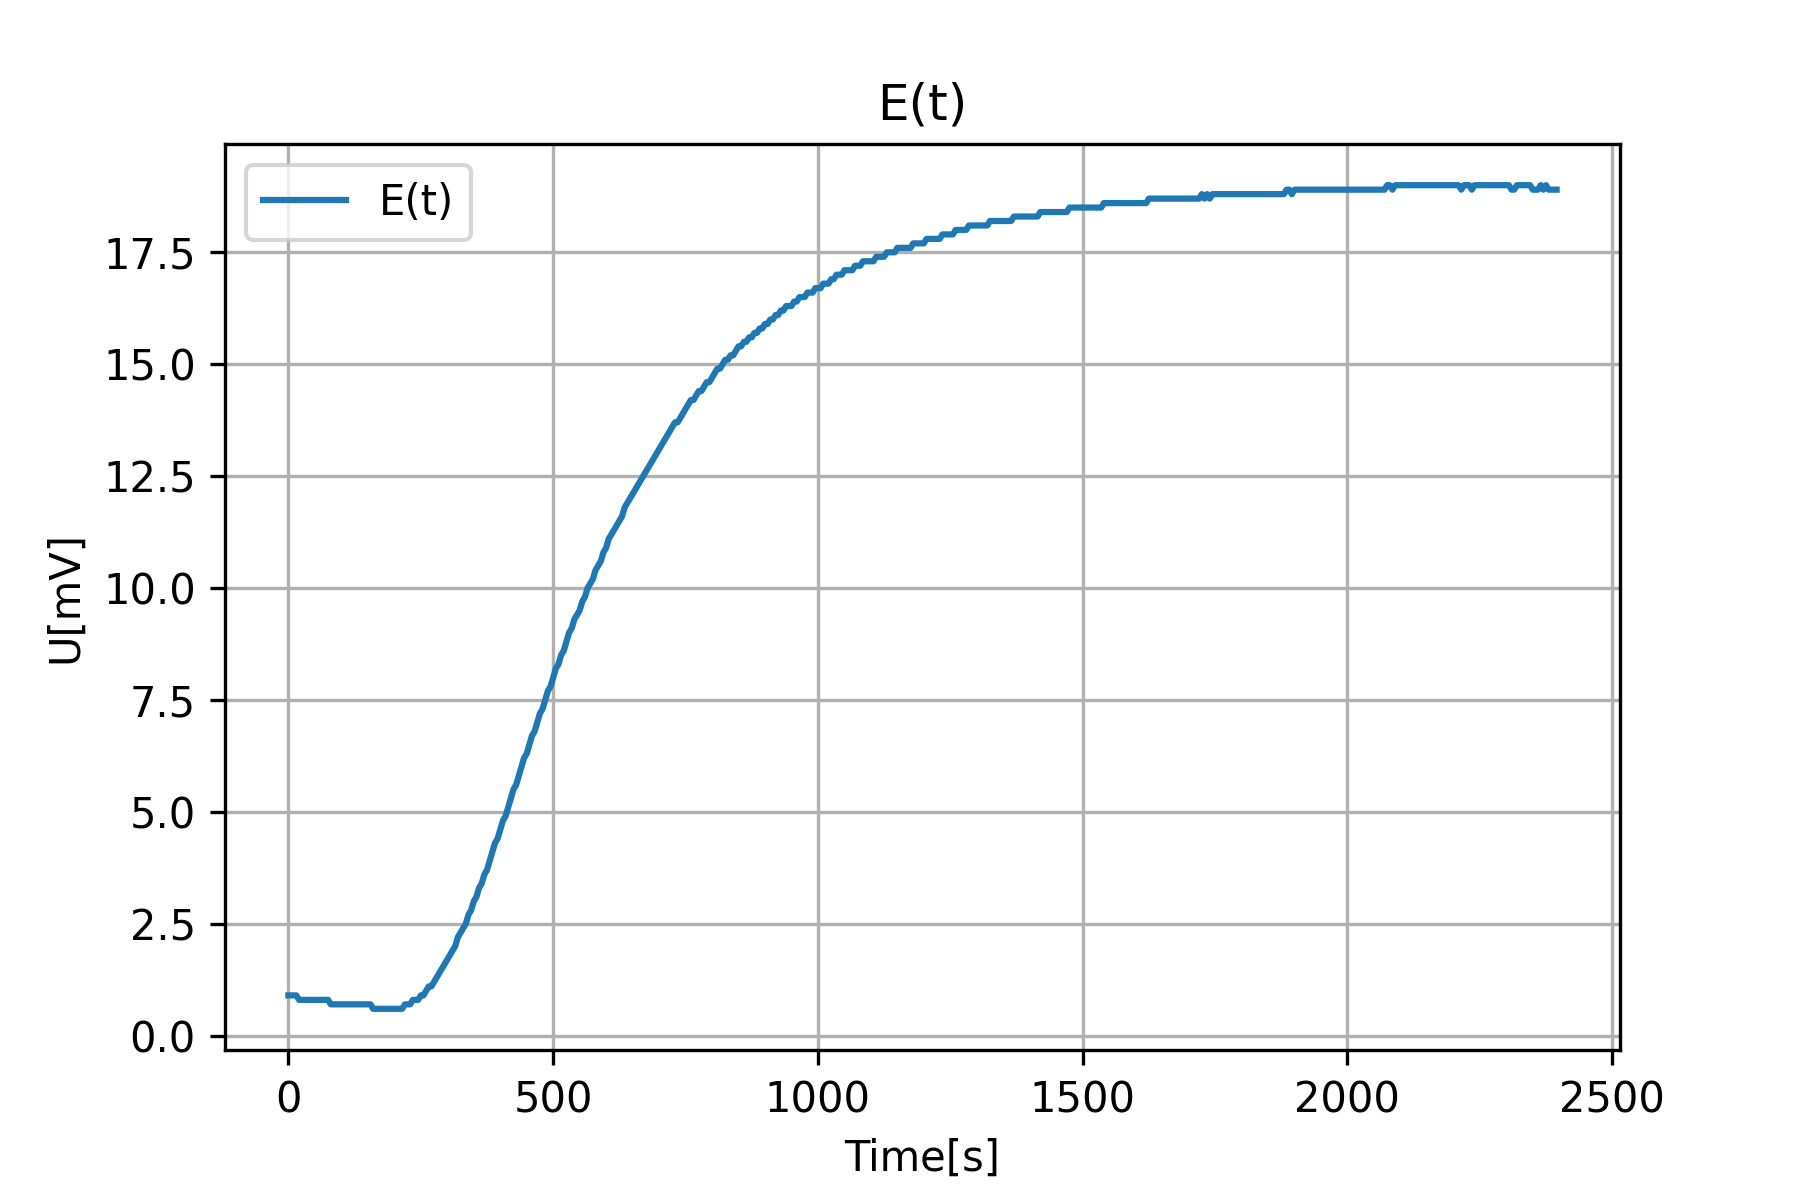
\includegraphics[scale=0.7]{oryginal.png}
\end{figure}

\newpage

\subsection{Kumpfmullera}
Na wyznaczonej charakterystyce naniesiono styczną przechodzącą przez punkt przegięcia A, następnie wyznaczono wartości $t_{i}, \ T_{m} \ i \ T_{z}$

\begin{figure}[h!]
    \centering
    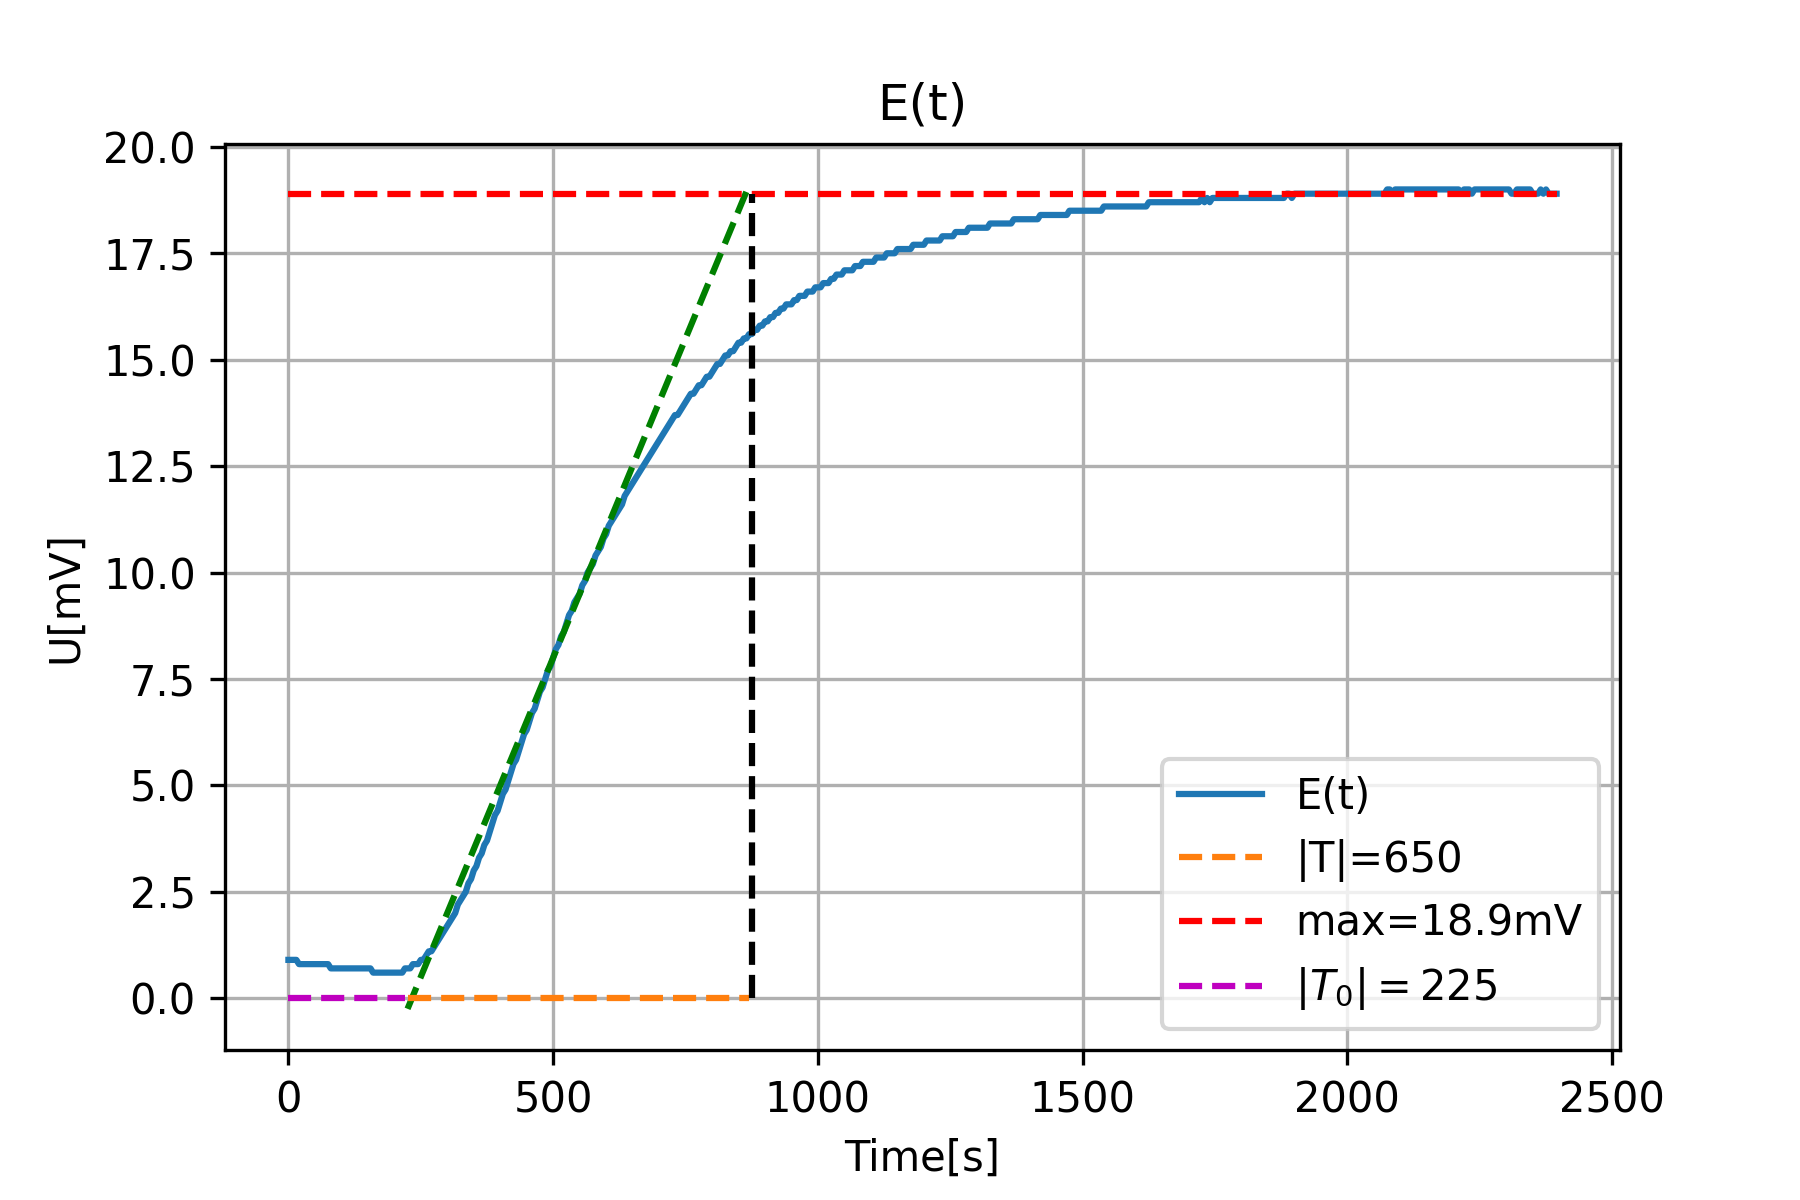
\includegraphics[scale=0.7]{oryginal_z_kreskami.png}
\end{figure}

Wzór na model zastępczy Kupfmullera:
$$ K\left(s\right)=\frac{k}{\left(Ts+1\right)}\cdot e^{sT_{0}} $$



Wartość wspóczynnika k wynosi tak samo jak w modelu Strejca$k=18.9[mV]$
Pozostałe parametry możemy ponownie
odczytać bezpośrednio z wykresu.
Tak więc ostateczny model to:
$$ K\left(s\right)=\frac{18.9}{\left(650s+1\right)}\cdot e^{225s} $$
\newpage
Następnie otrzymalismy symulację modelu Kumpfmullera z simulinka:



\begin{figure}[h!]
    \centering
    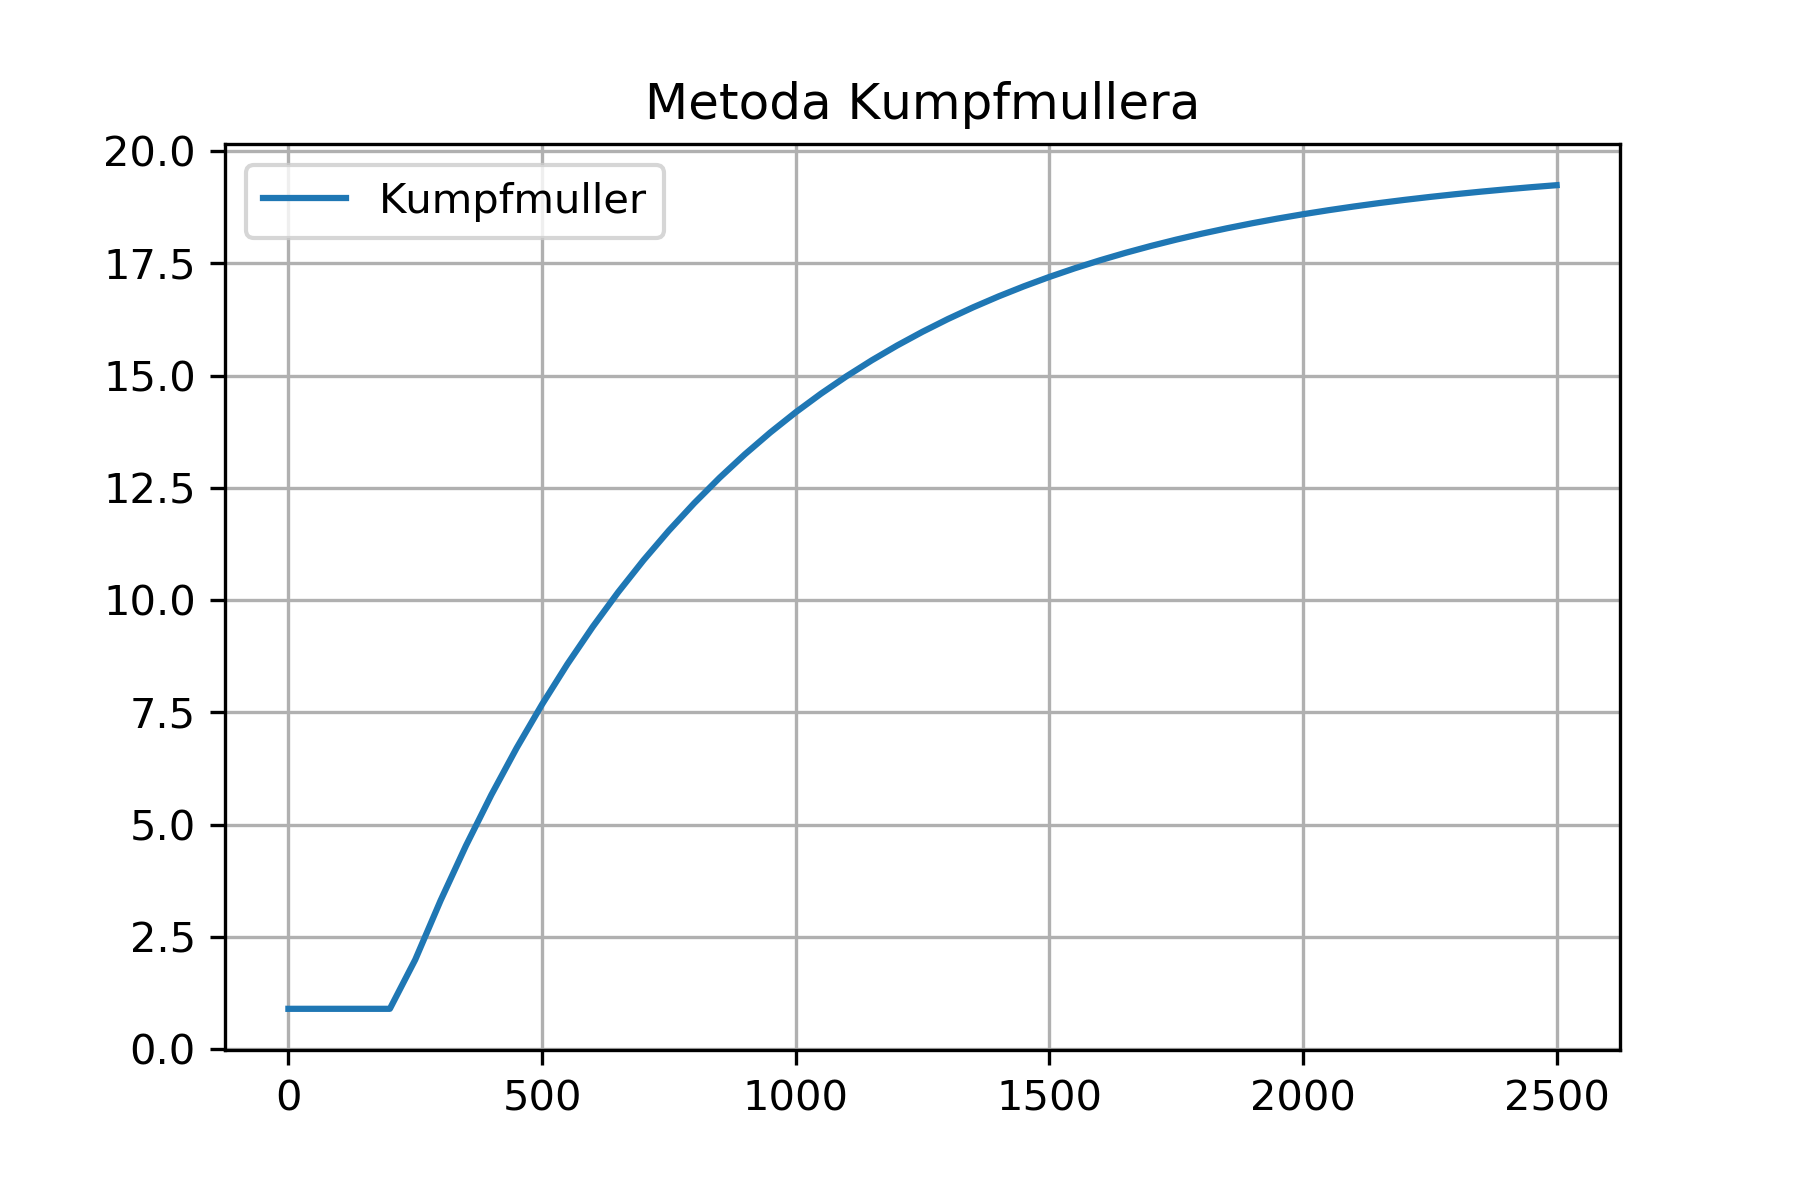
\includegraphics[scale=0.7]{metoda_kumpfmullera.png}
\end{figure}


\subsection{Strejca}

Odczytane wartosci z metody Strejca:

\[\begin{cases}
    T_{m}=T_{0}=255
    \\
    T_{z}=T=650
    \\
    k=18.9
\end{cases}\]

$$\tau = 
\left[
    \left(
        \frac{T_{m}}{T_{z}}
        -
        \frac{T_{m}}{T_{z}}
    \right)
\right]
\cdot
T_{z}\approx17.65$$

$$ t_{i}\approx207.35 $$

Główna postać:

$$ K\left(s\right)=\frac{18.9}{\left(650+1\right)} $$
Wykres otrzyany po symulacji:

\begin{figure}[h!]
    \centering
    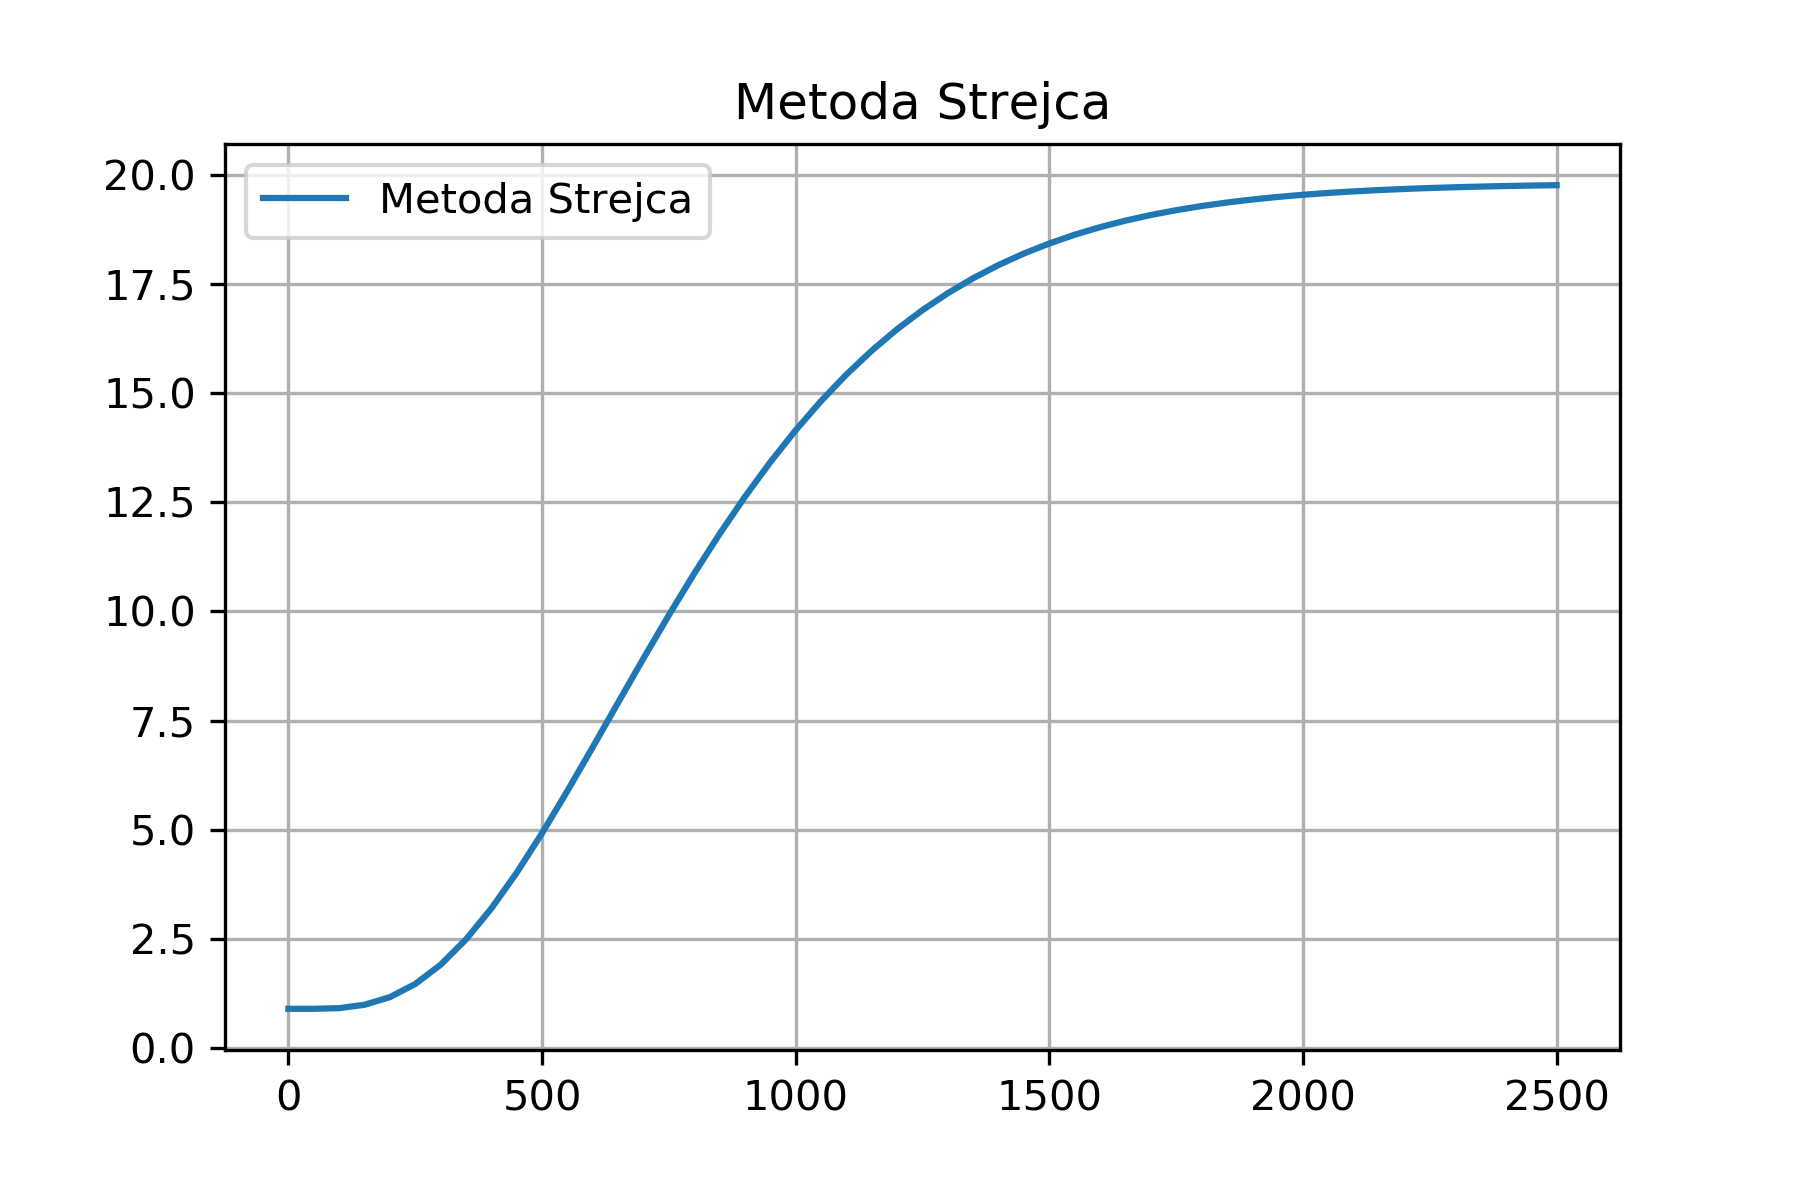
\includegraphics[scale=0.7]{metoda_strejca.png}
\end{figure}


\newpage

\subsection{Porównanie}
Symulacja w simulinku do obu metod:
\begin{figure}[h!]
    \centering
    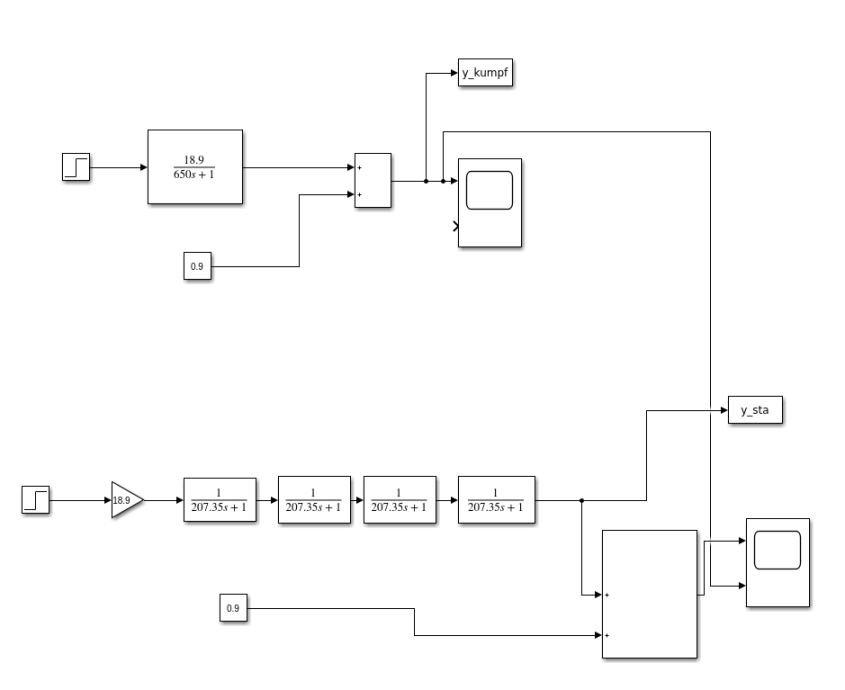
\includegraphics[scale=0.4]{sim.png}
\end{figure}

\begin{figure}[h!]
    \centering
    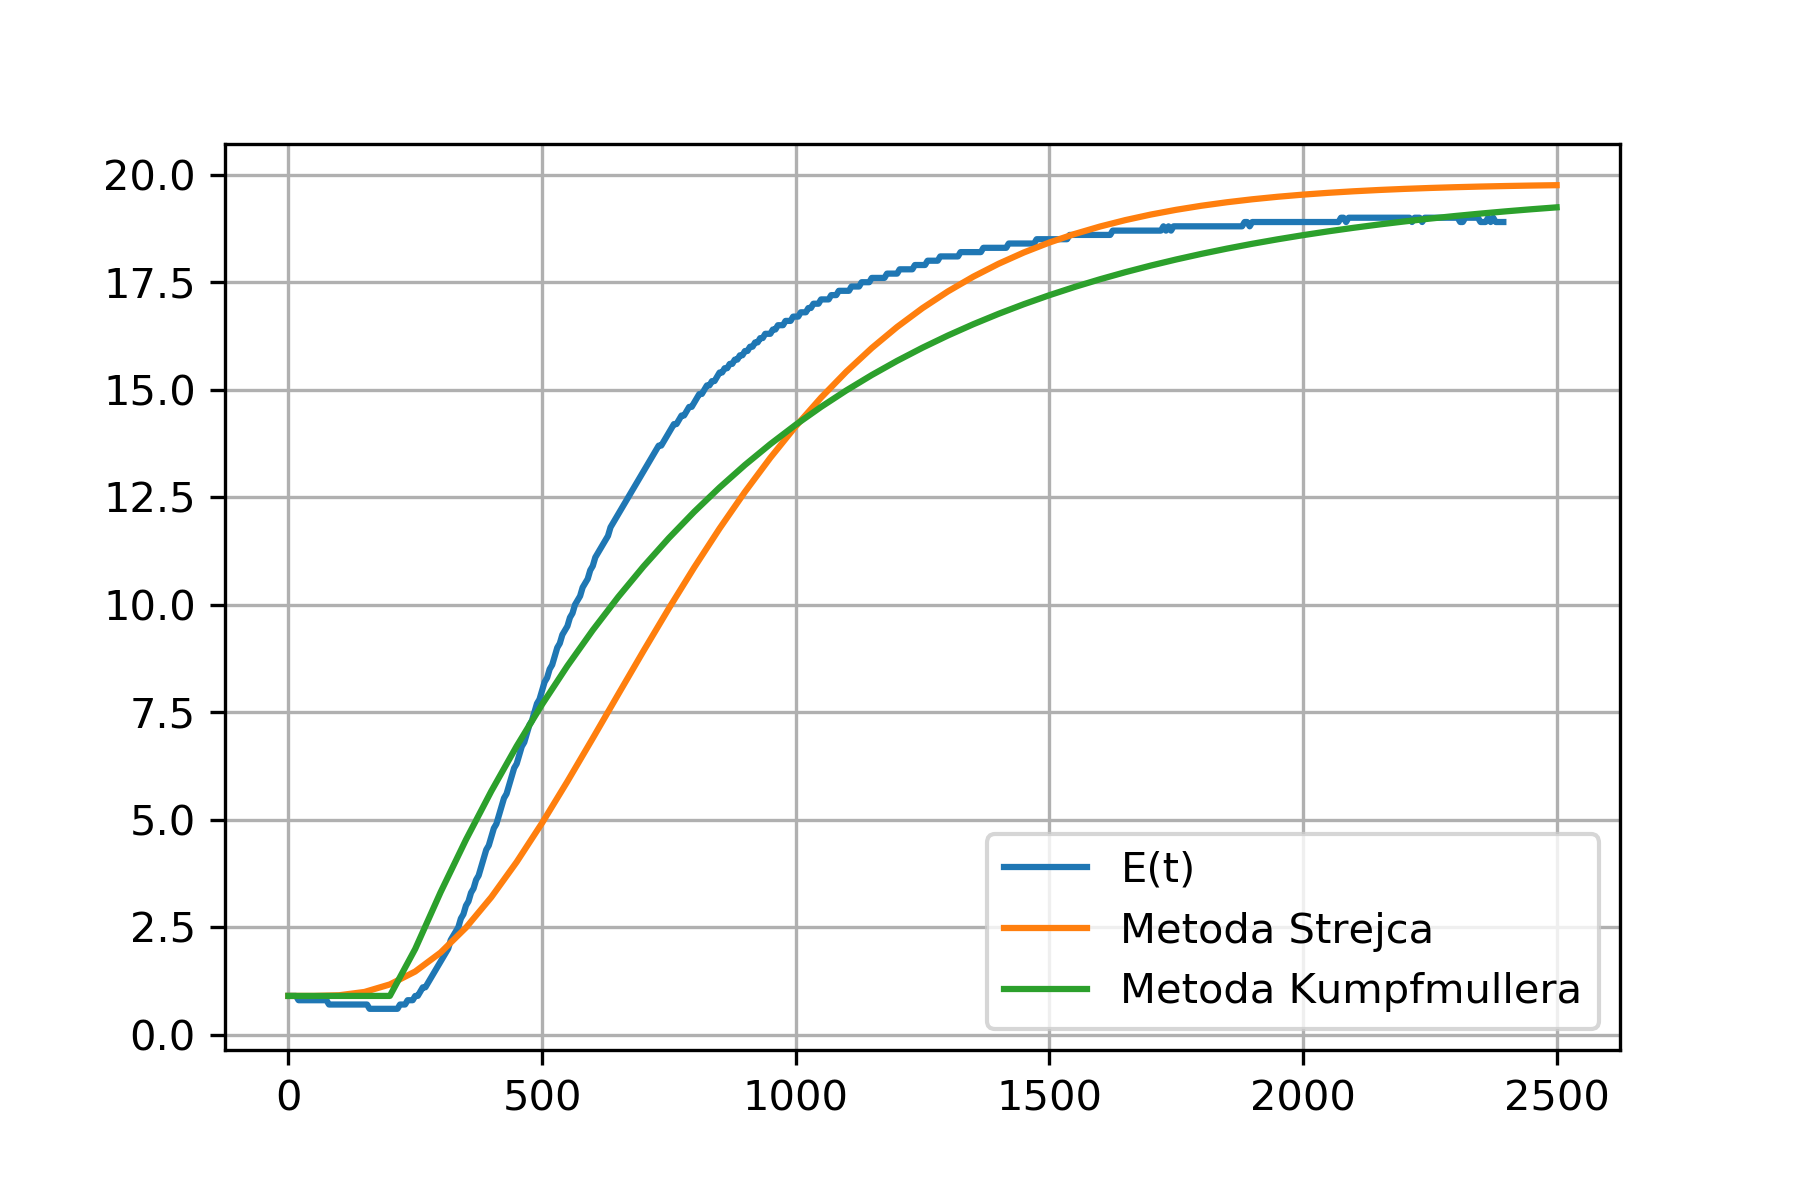
\includegraphics[scale=0.7]{metoda_porownanie.png}
\end{figure}

\section{Pytanie}
\subsection{Co mierzy termoelement?}
Termoelement najczęściej jest wykorzystywany jako czujnik temperatury, rzadziej jako źródło zasilania o bardzo niskim
napięciu i wysokim prądzie. Warunkiem działania termoelementu jest różnica temperatur na jego przeciwległych końcach,
pownieaż wykorzystuje on zjawisko generowania siły termoelektrycznej na styku dwóch różnych metali. Termoelement
mierzy różnice napięć, która powstaje w skutek zmiany temperatury na jego końcach.

\subsection{Do czego służą przewody kompensacyjne? Z czego są zbudowane?}
Przewody kompensacyjne są przystosowane do łączenia urządzeń pomiarowych z czujnikami termoelektrycznymi. Zbudo-
wany jest on z rdzenia (ten sam materiał co termopara) i izolacji wykonanej z tworzywa sztucznego. Niektóre typy są
dodatkowo wzmocnione włóknem szklanym lub cynkowym, aby zabezpieczyć przewód przed przerwaniem i rozciąganiem.

\subsection{Jak zidentyfikować czujnik pomiarowy temperatury w obiekcie przy pomocy multimetru i bez załączania zasilania obiektu?}

Czujnik podłączyć do obiektu o innej temperaturze niż temperatura odniesienia dla czujnika, a następnie za pomocą mul-
timetru zmierzyć napięcie i porównać jego wartość z tabelą wartości siły termoelektrycznej SME (mV) między spoinami.

\subsection{Jaki parametr zmienia się w tensometrze?}

Tensometr to miernik służący do pomiaru naprężenia. W praktyce mierzy się odkształcenie i oblicza naprężenie w oparciu
o przyjęty związek fizyczny.

\subsection{Jakie są warunki pomiaru prędkości obrotowej przy pomocy prądnicy tachometrycznej prądu stałego?}

Pomiar prędkości obrotu za pomocą prądnicy tachometrycznej wymaga sprzężenia osi prądnicy z wirującym elementem,
którego prędkość chcemy zmierzyć. Sygnał wyjściowy prądnicy tachometrycznej duży wpływ ma temperatura samej prąd-
nicy jak i obciążenie przyłożone do wyjścia, dlatego dobrą praktyką jest, aby prądnice były podłączane do układów o
bardzo dużej impedancji wejściowej.

\section{Wnioski}

Modele zastępcze takie jak Strejca czy Küpfmüllera mogą znacząco uprościć matematyczne opisy bardziej skomplikowanych
obiektów, dlatego tak ważna jest ich jak najdokładniejsze odwzorowanie rzeczywistego obiektu. Zależy to w dużej mierze
od poprawnego odczytania ich parametrów z charakterystyk dynamicznych rzeczywistych obiektów przez osobę za to
odpowiedzialną.

\end{document}
